

\documentclass[a4paper,12 pt]{article}
\usepackage{graphicx}
\usepackage{caption}
\usepackage{refstyle}
\usepackage{wrapfig}
\usepackage{subcaption}
\usepackage{geometry}
 \geometry{
 a4paper,
 total={210mm,297mm},
 left=25mm,
 right=25mm,
 top=25mm,
 bottom=25mm,
 }

\title {Project Report \\ Sensor Module Interfacing \\[10pt] Task:
Interfacing Accelerometer MMA7361 with ATmega2560 in Firebird V Robot \\[25pt] Team members }
\author {Chayatan \and Mukilan A \and Shantanu}

\begin{document}
\maketitle
\begin{center}
\begin{large}
Under the guidance of\\
\textbf{Prof. Kavi Arya\\and\\Parin Chedda}\\
\vspace{0.5in}
\end{large}
\end{center}
\begin{center}

\includegraphics[scale=0.32]{iitb.png}
\end{center}
\begin{center}
\begin{large}
Embedded and Real-Time Systems Laboratory \\
Department of Computer Science and Engineering \\
Indian Institute of Technology \\
Bombay \\
\end{large}
\end{center}

\newpage
\tableofcontents
\newpage

\begin{abstract}
The project aims at interfacing an accelerometer sensor with Fire Bird
V educational robot. This additional module can be used for detection
of the degree of tilt of the module. In this
paper we will see about the basic  MMA7361 Accelerometer sensor
module interfacing with Atmega 2560 in Fire Bird V robot. This will
include the working principle, basic interfacing circuit, programming and
applications of the MMA7361 Accelerometer.
\end{abstract}

\section{Introduction}
\ \ As the name indicates this sensor is used to measure acceleration. Acceleration here does not mean rate of change in velocity in a particular axis. This sensor instead provides the ‘g’ force that is acting on the test mass located inside the sensor. The measure of force that each coordinate experiences due to the action of gravity is what the sensor actually measures. 
	For example, an accelerometer at rest on the surface of the earth will measure an acceleration g= 9.81 m/s2 straight upwards, due to its weight. By contrast, accelerometers in free fall or at rest in outer space will measure zero. The term for the type of acceleration that accelerometers can measure is g-force acceleration.

\section{How an Accelerometer Works } 
\vspace {5 mm}
\begin{figure}[h]
\begin{center}
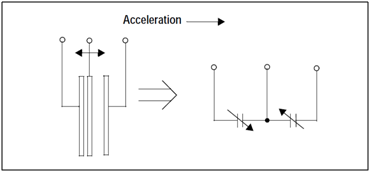
\includegraphics[]{gcell.png}
\caption{Structure of a g-Cell}
\label{fig:1}
\end{center}
\end{figure}
\vspace{-20 pt}
The Freescale accelerometer is a surface-micromachined integrated-circuit accelerometer. The device consists of a surface micromachined capacitive sensing cell (g-cell) and a signal conditioning ASIC contained in a single package.


The g-cell is a mechanical structure, as shown in \figref{1}, formed from semiconductor materials (polysilicon) using semiconductor processes (masking and etching). It can be modeled as a set of beams attached to a movable central mass that move between fixed beams. The movable beams can be deflected from their rest position by subjecting the system to an acceleration. As the beams attached to the central mass move, the distance from them to the fixed beams on one side will increase by the same amount that the distance to the fixed beams on the other side decreases. The change in distance is a measure of acceleration. The g-cell beams form two back-to-back capacitors. As the center beam moves with acceleration, the distance between the beams changes and each capacitor's value will change, (C = Aε/D). Where A is the area of the beam, ε is the dielectric constant, and  D is the distance between the beams.

%----------------------------------------------------------------------------------------------------------------
\pagebreak

\section{Pin Connections of MMA7361 Accelerometer }
\vspace {5 mm}
\begin{figure}[h]
\begin{center}
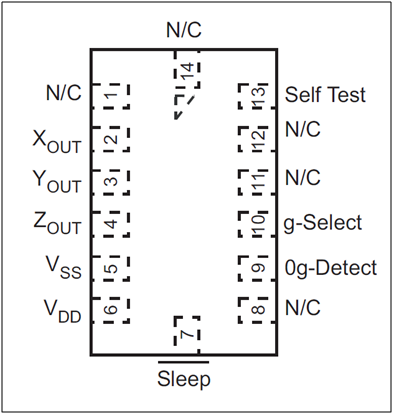
\includegraphics[]{acc1.png}
\caption{Pin Diagram}
\label{fig:2}

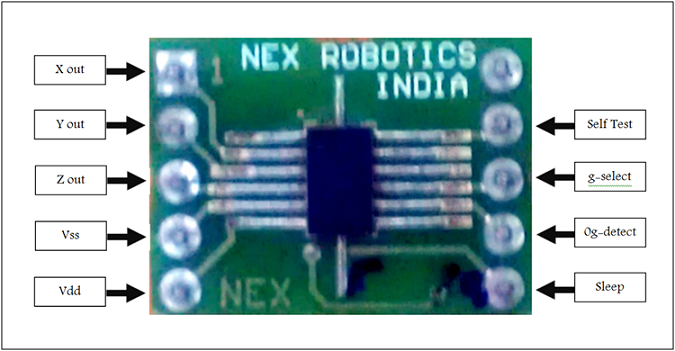
\includegraphics[]{acc2.png}
\caption{Pin Connections of the Accelerometer}
\label{fig:3}
\end{center}
\end{figure}
%----------------------------------------------------------------------------------------------------------------

\pagebreak
\section{Connections of MMA7361 Accelerometer with the ATmega2560}
\vspace {5 mm}
\begin{enumerate}

\item Connect the Xout, Yout, and Zout pins to the PORT K pins (analog channels ) of the ATmega2560 processor to convert the analog output values of the Accelerometer to digital values that can be used by the Microcontroller.
\item Connect the Vss Pin of the accelerometer to the Ground pin of the Microcontroller.
\item Connect the Vdd Pin of the accelerometer to the 3.3V of the Microcontroller.
\item The Sleep pin is shorted to the Vdd pin of the Accelerometer, in order to provide significant reduction in the operating current.
\item The remaining pins of the accelerometer i.e. Self Test, G select, 0g detect pins are left unconnected because
\begin{itemize}

\item  0g detect pin is an output pin which gives high output if all the x, y, z axes are at 0g.
\item Self Test pin allows the verification of the mechanical and electrical integrity of the accelerometer at any time before or after installation.
\item G select pins are left open because the operation of the accelerometer is in the 0g mode, where the sensitivity is 800mv/g.
\end{itemize}
\end{enumerate}

\begin{figure}[!h]
\begin{center}
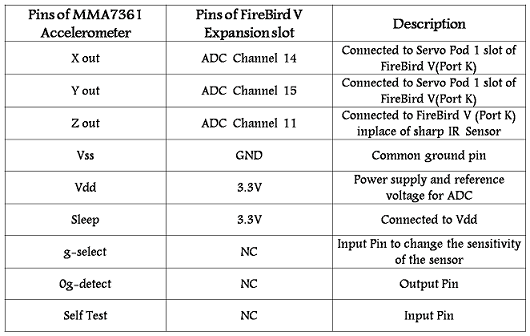
\includegraphics[]{Picture1.png}
\caption{Connections of MMA7361 Accelerometer with the ATmega2560}

\end{center}
\end{figure}
\pagebreak
%----------------------------------------------------------------------------------------------------------------
\section{Orientation of the Accelerometer along the Various Axes}
\vspace {5 mm}
\begin{figure}[h]
\begin{center}
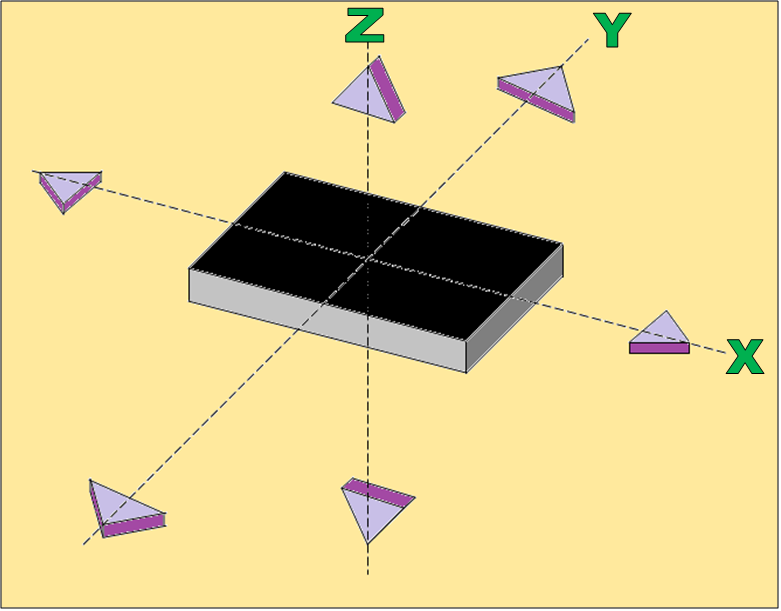
\includegraphics[]{acc3.png}
\caption{Orientation of the Accelerometer along the Various Axes}
\label{fig:4}
\end{center}
\end{figure}
\pagebreak
%----------------------------------------------------------------------------------------------------------------
\section{Table showing the values of the Accelerometer along the Various Axes}

\begin{figure}[!h]
\begin{center}
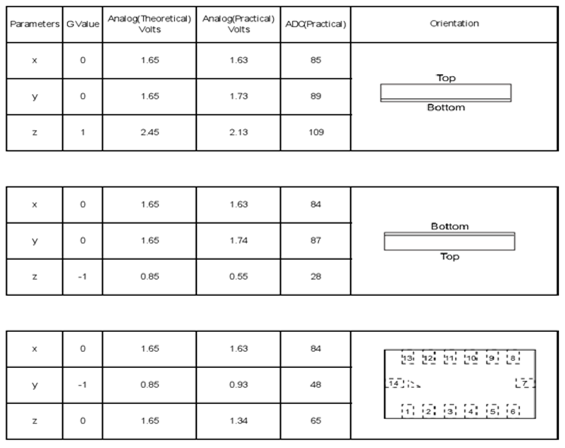
\includegraphics[]{acc4.png}
\label{fig:5}
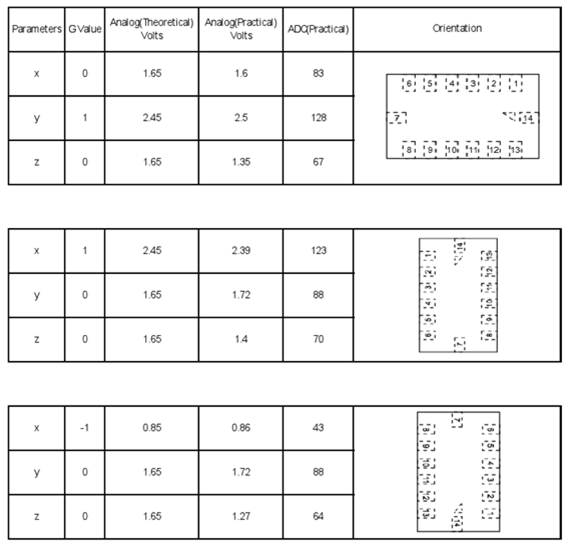
\includegraphics[]{acc5.png}
\label{fig:6}
\end{center}
\end{figure}
\pagebreak
%----------------------------------------------------------------------------------------------------------------


\section{C Code}
\subsection{Using the header file}
As explained earlier, this sensor, senses orientation of the particular axis and accordingly gives the analog output on the Xout, Yout and Zout pins.\\
Therefore we have defined a header file called as \textbf{accelerometer.h} where we call the following functions that are used in interfacing the Accelerometer to the Firebird V Robot.
This header file can be found in the \textbf{Headers} folder.\\
The following functions are used in this header file:\\

\begin{itemize}
\item \begin{verbatim}
acc_init_devices() function : This function initializes all the
 ADC ports and configures the respective ADC registers.
\end{verbatim}
\end{itemize}

\begin{itemize}
\item	\begin{verbatim}
acc_process() : This function is used to compare the ADC values
 with the threshold, make the oriental decision and updates the
 left, right, forward and backward flags.
\end{verbatim}
\end{itemize}

\begin{itemize}
\item	\begin{verbatim}
acc_get_x() : This function will get the ADC values of the 
X co-ordinate of the Accelerometer when connected to the ADC
\end{verbatim}
\end{itemize}

\begin{itemize}
\item	\begin{verbatim}
acc_get_y() : This function will get the ADC values of the 
Y co-ordinate of the Accelerometer when connected to the ADC
\end{verbatim}
\end{itemize}

\begin{itemize}
\item	\begin{verbatim}
acc_get_z() : This function will get the ADC values of the 
Z co-ordinate of the Accelerometer when connected to the ADC
\end{verbatim}
\end{itemize}




These functions will be explained in detailed in the later sections.

\subsection{Sample code calling the accelerometer.h header file}
Now we will see the Sample Program calling the scan pir.h header. Prior to the C Code, The following
connections should be made:

\begin{figure}[!h]
\begin{center}
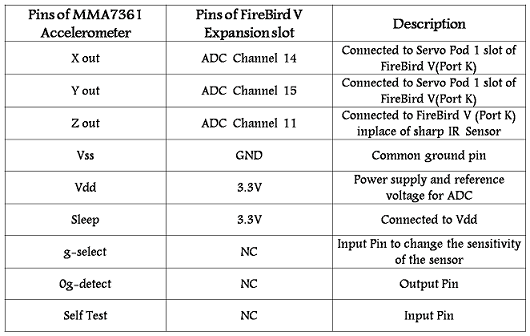
\includegraphics[scale=0.65]{Picture1.png}
\caption{Connections of MMA7361 Accelerometer with the ATmega2560}

\end{center}
\end{figure}
\newpage
\begin{center}
\LARGE{\textbf{SAMPLE CODE}}
\end{center}
\large 
\begin{verbatim}
#define F_CPU 14745600
#include <avr/io.h>
#include <avr/interrupt.h>
#include <util/delay.h>
#include <math.h>
#include "lcd.h"
#include "accelerometer.h"

int main(void)
{
	
	unsigned char x,y,z;     //Initialise variables
	acc_init_devices();      //Initialise the Ports for LCD & ADC
	lcd_cursor(2,8);
	
	while(1)
	{
		acc_process();    //Read the ADC values of the
                  //Accelerometer connected to the ADC pins
		x=acc_get_x();             //Get X Co-ordinate values
		y=acc_get_y();             //Get Y Co-ordinate values
		z=acc_get_z();             //Get Z Co-ordinate values
		lcd_print(2,1,x,3);        //Display the X value in LCD  
lcd_print(2,6,y,3);        //Display the Y value in LCD
lcd_print(2,11,z,3);       //Display the Z value in LCD
 
	}		
return 0;
}

\end{verbatim}
%-----------------------------------------------------------------------------
\newpage
\subsection{Functions used in the accelerometer.h header file}
\begin{enumerate}
\item \textbf{acc\_init\_devices() :}\\
\vspace{-5mm}
\begin{verbatim}
void acc_init_devices()
{
	cli();           //Clear Interrupt
	port_init();     //Initialise the ADC & LCD Port pins
	lcd_init();      //Initialise LCD 
	adc_init();      //Initialise ADC
	sei();           //Clear Interrupt
}

\end{verbatim}

\item \textbf{acc\_init\_devices() :}\\
\vspace{-5mm}
\begin{verbatim}
void acc_process(void)
{
	x= ADC_Conversion(14);  //ADC Conversion of X out
	y= ADC_Conversion(15);  //ADC Conversion of Y out
	z= ADC_Conversion(11);  //ADC Conversion of Z out

//The code below can be uncommented to check if the
//values obtained by the ADC for the Accerometer are
// accurate or not

	/*
lcd_cursor(1,1);
	lcd_string("X = ");
	lcd_print(1,4,x,3);
	lcd_cursor(1,7);
	lcd_string(" y = ");
	lcd_print(1,11,y,3);
	lcd_cursor(2,1);
	lcd_string("z = ");
	lcd_print(2,4,z,3)
;*/

}


\end{verbatim}

\item \textbf{acc\_get\_x() :}\\
\vspace{-5mm}
\begin{verbatim}
unsigned char acc_get_x(void)
{
	return(x);     //return the value of x
}

\end{verbatim}

\item \textbf{acc\_get\_y() :}\\
\vspace{-5mm}
\begin{verbatim}
unsigned char acc_get_y(void)
{
	return(y);     //return the value of y
}

\end{verbatim}


\item \textbf{acc\_get\_z() :}\\
\vspace{-5mm}
\begin{verbatim}
unsigned char acc_get_z(void)
{
	return(z);     //return the value of z
}

\end{verbatim}

\end{enumerate}

\pagebreak
\section{Sample Output as seen on LCD}

\begin{figure}[!h]
\begin{center}
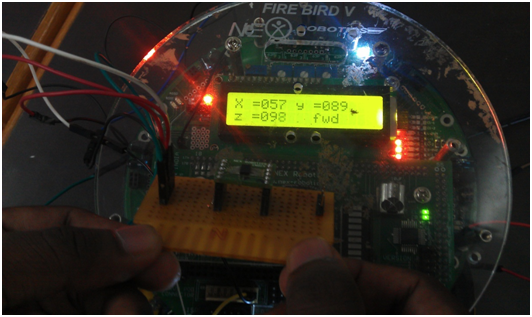
\includegraphics[]{acco1.png}
\label{fig:7}
\vspace{7mm}
\caption{LCD Sample Output : Forward}
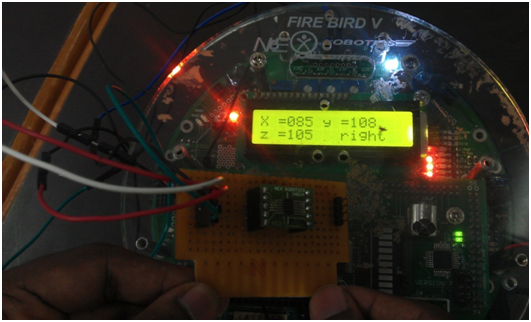
\includegraphics[]{acco2.png}
\label{fig:8}
\caption{LCD Sample Output : Right}
\end{center}
\end{figure}

\pagebreak

\begin{figure}[!h]
\begin{center}
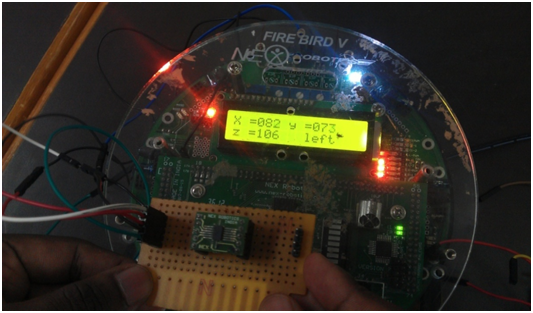
\includegraphics[]{acco3.png}
\label{fig:9}
\caption{LCD Sample Output : Left}
\vspace{7mm}
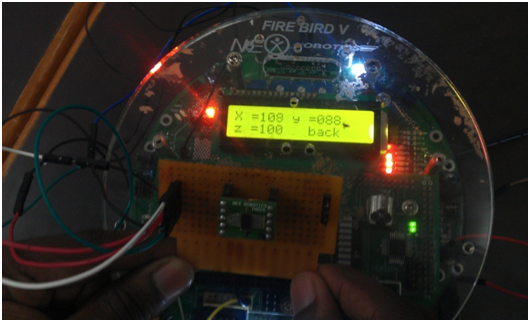
\includegraphics[]{acco4.png}
\caption{LCD Sample Output : Back}
\label{fig:10}
\end{center}
\end{figure}
\pagebreak

%-----------------------------------------------------------------------------

\section{Applications}

\begin{itemize}
\item Currently used in :
\begin{itemize}
\item Mobiles and iPods for changing orientation from Landscape to Portrait mode or vice versa.
\item Gaming for motion sensing
\item Protect laptops and mobiles when under free fall
\item Vehicles to detect collision and deploy airbags.
\item As an alternative to spirit level for balancing.
\end{itemize}
\item Future Uses :

\begin{itemize}
\item Can be used for simulating driver training, in which a steering wheel including an accelerometer will turn the vehicle on the screen according to the tilt provided. This would enable safe driving practice with any dangers of collision.
\item For Robot Movement similar to the walking support system as shown in the picture \figref{11}

\item Accelerometers measuring dynamic forces such as vibrations can be used for designing Virtual Keyboards as shown in 10b
\begin{figure}[h]
        \centering
        \begin{subfigure}[b]{0.55\textwidth}
                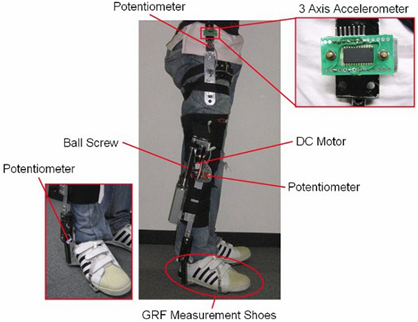
\includegraphics[width=\textwidth]{accapp.png}
                \caption{Walking Support System}
                \label{fig:11}
        \end{subfigure}%
        \begin{subfigure}[b]{0.40\textwidth}
                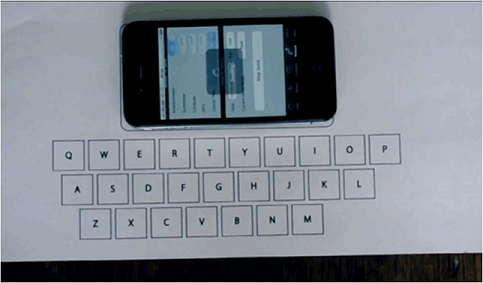
\includegraphics[width=\textwidth]{accapp1.png}
                \caption{Virtual Keyboard Concept}
                \label{fig:12}
        \end{subfigure}%

        
\end{figure}
\end{itemize}
\end{itemize}

\pagebreak
\end{document}